\begin{figure}
    \begin{center}
    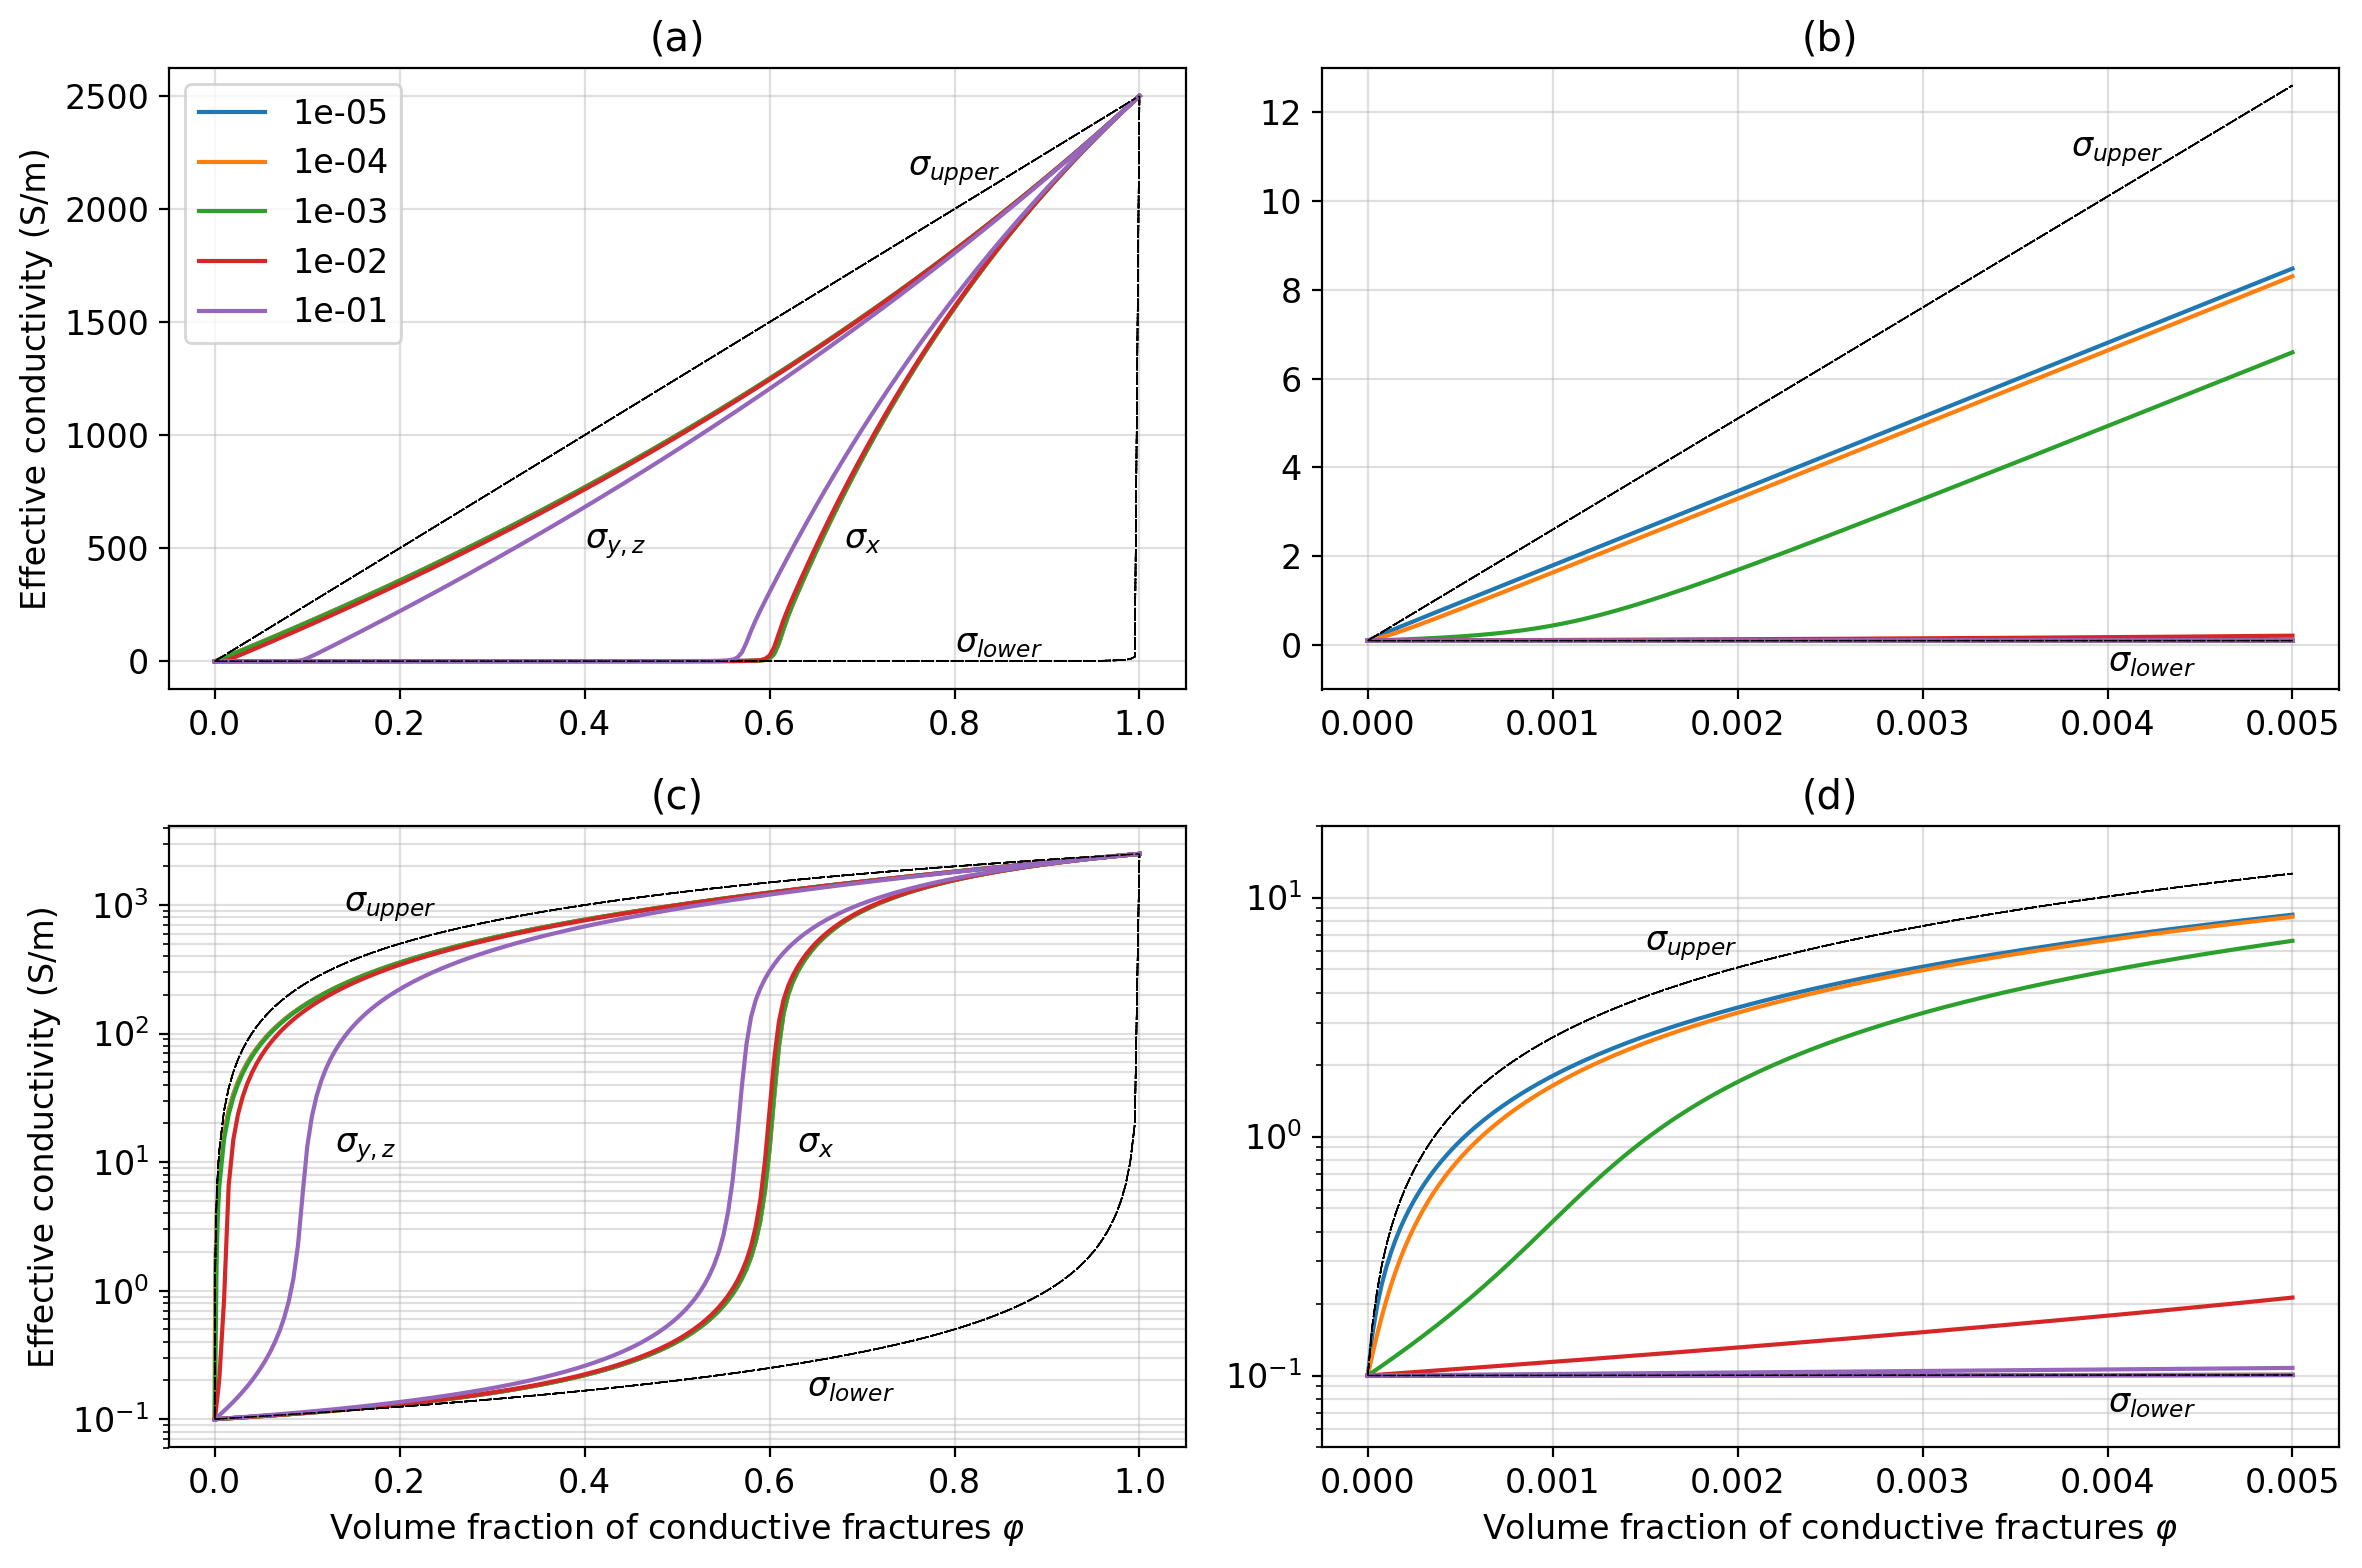
\includegraphics[width=\columnwidth]{figures/phys_prop_model/aligned_fractures.png}
    \end{center}
\caption{
    Effective, anisotropic conductivity for a fractured rock with spheroidal
    cracks whose normal is oriented along the y-axis for five different aspect ratios, indicated by the legend.
    The black dashed lines show the upper and lower
    Wiener Bounds, which are identical the volume-weighted arithemtic and harmonic averages of the
    conductivity of the rock (0.1 S/m) and proppant-fluid mixture (2500 S/m). The black dash-dot lines
    are the anisotropic Hashin-Shtrikman upper and lower bounds computed using an aspect ratio of $10^{-5}$ in
    equation \ref{eq:hashin_shtrikman_bounds_anisotropic}.
    Panel (a) shows the
    full range $0 \leq \varphi \leq 1$, and panel (b) zooms in to $0 \leq \varphi \leq 0.005$.
    Note that in (b), any curve that deviates from the lower bound is the $\sigma_{x, z}$ component;
    all $\sigma_x$ values lie on the lower bound for the concentration range shown.
}
\label{fig:aligned_fractures}
\end{figure}
